\documentclass{article}
\usepackage{amsmath}
\usepackage{listings}
\usepackage{xcolor}
\usepackage{graphicx}
\usepackage{geometry}
\usepackage{hyperref}
\usepackage{tikz}
\usetikzlibrary{trees, positioning}
\geometry{margin=1in}

\title{Sorting}
\author{}
\date{}

\definecolor{codegray}{rgb}{0.5,0.5,0.5}
\definecolor{backcolour}{rgb}{0.95,0.95,0.92}

\lstdefinestyle{cppstyle}{
  backgroundcolor=\color{backcolour},
  commentstyle=\color{codegray},
  keywordstyle=\color{blue},
  numberstyle=\tiny\color{codegray},
  stringstyle=\color{red},
  basicstyle=\ttfamily\footnotesize,
  breakatwhitespace=false,
  breaklines=true,
  captionpos=b,
  keepspaces=true,
  numbers=none,
  numbersep=5pt,
  showspaces=false,
  showstringspaces=false,
  showtabs=false,
  tabsize=2,
  language=C++
}

\begin{document}

\maketitle



Sorting is the process of arranging elements in a specific order, typically in ascending or descending numerical or lexicographical order. It is a fundamental operation in computer science with applications in searching, data analysis, and algorithm optimization.

Efficient sorting improves the performance of other algorithms that require sorted input, such as binary search or merge-based algorithms. 

\section{Bubble Sort}
Bubble Sort repeatedly steps through the list, compares adjacent elements and swaps them if they are in the wrong order.

\begin{lstlisting}[style=cppstyle]
// Bubble Sort
void bubbleSort(int arr[], int n) {
    for (int i = 0; i < n - 1; ++i)
        for (int j = 0; j < n - i - 1; ++j)
            if (arr[j] > arr[j + 1])
                std::swap(arr[j], arr[j + 1]);  // Swap if out of order
}
\end{lstlisting}

Time complexity: $O(n^2)$
Space complexity: $O(1)$

\section{Insertion Sort}
Insertion Sort builds the sorted array one item at a time by comparing and inserting the current element at the right position.

\begin{lstlisting}[style=cppstyle]
// Insertion Sort
// Sorts arr[] of size n in ascending order by inserting each element into its correct position
void insertionSort(int arr[], int n) {
    // Start from the second element (index 1), as the first element is trivially sorted
    for (int i = 1; i < n; ++i) {
        int key = arr[i];        // The element to insert into the sorted portion
        int j = i - 1;           // Index of the last element in the sorted portion

        // Shift elements in the sorted portion that are greater than key to the right
        while (j >= 0 && arr[j] > key) {
            arr[j + 1] = arr[j]; // Move element one position to the right
            --j;                 // Move to the next element on the left
        }

        // Insert key at its correct position
        arr[j + 1] = key;
    }
}
\end{lstlisting}

Time complexity: $O(n^2)$
Space complexity: $O(1)$

\section{Selection Sort}
Selection Sort repeatedly finds the minimum element from the unsorted part and puts it at the beginning.

\begin{lstlisting}[style=cppstyle]
// Selection Sort
// Sorts arr[] of size n in ascending order by selecting the minimum element at each step
void selectionSort(int arr[], int n) {
    // Move the boundary of the unsorted subarray one by one
    for (int i = 0; i < n - 1; ++i) {
        int min_idx = i; // Assume the current position has the minimum

        // Find the minimum element in the unsorted subarray
        for (int j = i + 1; j < n; ++j) {
            if (arr[j] < arr[min_idx]) {
                min_idx = j;
            }
        }

        // Swap the found minimum element with the first element of the unsorted part
        std::swap(arr[min_idx], arr[i]);
    }
}
\end{lstlisting}

Time complexity: $O(n^2)$
Space complexity: $O(1)$

\section{Merge Sort}
Merge Sort is a divide-and-conquer algorithm that divides the array into halves, sorts them recursively, and merges them.

\begin{lstlisting}[style=cppstyle]
// Merge two sorted halves: arr[l..m] and arr[m+1..r]
void merge(int arr[], int l, int m, int r) {
    int n1 = m - l + 1;    // Size of left subarray
    int n2 = r - m;        // Size of right subarray
    int L[n1], R[n2];      // Temporary arrays

    // Copy data to temp arrays L[] and R[]
    for (int i = 0; i < n1; ++i)
        L[i] = arr[l + i];
    for (int j = 0; j < n2; ++j)
        R[j] = arr[m + 1 + j];

    int i = 0, j = 0, k = l;

    // Merge the temp arrays back into arr[l..r]
    while (i < n1 && j < n2) {
        if (L[i] <= R[j])
            arr[k++] = L[i++];
        else
            arr[k++] = R[j++];
    }

    // Copy remaining elements of L[], if any
    while (i < n1)
        arr[k++] = L[i++];

    // Copy remaining elements of R[], if any
    while (j < n2)
        arr[k++] = R[j++];
}

// Merge Sort: sorts arr[l..r] using merge()
void mergeSort(int arr[], int l, int r) {
    if (l < r) {
        int m = l + (r - l) / 2; // Avoid overflow

        // Sort first and second halves
        mergeSort(arr, l, m);
        mergeSort(arr, m + 1, r);

        // Merge the sorted halves
        merge(arr, l, m, r);
    }
}
\end{lstlisting}

\subsection{Merge Sort and the Master Method}

Merge Sort uses a divide-and-conquer approach. It divides the array into two halves, recursively sorts each half, and then merges them. Its time recurrence is:

\[
T(n) = 2 \cdot T\left(\frac{n}{2}\right) + O(n)
\]

This fits the general divide-and-conquer form:

\[
T(n) = a \cdot T\left(\frac{n}{b}\right) + f(n)
\]

with parameters:
\begin{itemize}
    \item $a = 2$ (number of subproblems),
    \item $b = 2$ (each subproblem is half the size),
    \item $f(n) = O(n)$ (cost of merging two sorted subarrays).
\end{itemize}

Let $d = 1$ since $f(n) = O(n^1)$, and compute:

\[
c = \log_b a = \log_2 2 = 1
\]

We now compare $d$ and $c$:
\begin{itemize}
    \item Since $d = c = 1$, this is \textbf{Case 2} of the Master Theorem.
\end{itemize}

By Case 2:
\[
T(n) = O(n^d \log n) = O(n \log n)
\]

The time complexity of Merge Sort is $O(n \log n)$, derived using the Master Method with $a = 2$, $b = 2$, and $f(n) = O(n^1)$.
Space complexity is $O(n)$

\section{Quick Sort}
Quick Sort picks a pivot element, partitions the array around the pivot, and sorts the partitions recursively.

\begin{lstlisting}[style=cppstyle]
// Partition function: places pivot at correct position
// and arranges smaller elements to the left and larger to the right
int partition(int arr[], int low, int high) {
    int pivot = arr[high];  // Choose the last element as pivot
    int i = low - 1;        // Index of smaller element

    // Traverse the array and rearrange elements
    for (int j = low; j < high; ++j) {
        if (arr[j] < pivot) {
            ++i;
            std::swap(arr[i], arr[j]);
        }
    }

    // Place pivot at its correct position
    std::swap(arr[i + 1], arr[high]);
    return i + 1;           // Return the partition index
}

// Quick Sort: recursively sorts arr[low..high]
void quickSort(int arr[], int low, int high) {
    if (low < high) {
        // Partition the array and get pivot index
        int pi = partition(arr, low, high);

        // Recursively sort elements before and after partition
        quickSort(arr, low, pi - 1);
        quickSort(arr, pi + 1, high);
  
\end{lstlisting}

\subsection*{Average-Case Complexity of Quick Sort}

Quick Sort is a divide-and-conquer algorithm that partitions an array around a pivot element such that elements less than the pivot go to the left subarray and greater elements to the right. It then recursively sorts each subarray.

The efficiency of Quick Sort depends heavily on the quality of the pivot selection. If the pivot splits the array into two equal halves at each step—i.e., is always the median—the recurrence becomes:

\[
T(n) = 2 \cdot T\left(\frac{n}{2}\right) + O(n)
\]

This is the same recurrence as Merge Sort and yields an overall time complexity of:

\[
T(n) = O(n \log n)
\]

However, unlike Merge Sort, Quick Sort does not guarantee a balanced split. The algorithm randomly selects pivots or uses heuristics (like picking the first or last element), making it a **probabilistic algorithm**.

In the average case, random pivots tend to split the input into reasonably balanced partitions on average. The expected depth of the recursion tree remains $O(\log n)$, and each level performs $O(n)$ work for partitioning. Hence, the expected total running time is:

\[
O(n \log n)
\]

Quick Sort runs in $O(n \log n)$ time on average due to its expected balanced partitions, though in the worst case (e.g., always picking the smallest or largest element as pivot), it degrades to $O(n^2)$. Space complexity is $O(1)$

\section{Heap Sort}
Heap Sort converts the array into a max heap and extracts the maximum repeatedly.

\begin{lstlisting}[style=cppstyle]
void heapSort(std::vector<int>& arr) {
    // Create a max heap
    std::priority_queue<int> pq;

    // Insert all elements into the priority queue
    for (int num : arr) {
        pq.push(num);
    }

    // Extract elements from the heap and store in reverse order
    for (int i = arr.size() - 1; i >= 0; --i) {
        arr[i] = pq.top();
        pq.pop();
    }
}
\end{lstlisting}

To sort in ascending order using a **min-heap**, reverse the order of extraction or use a custom comparator:

\begin{lstlisting}[style=cppstyle]
// Min-heap using greater<int> comparator
std::priority_queue<int, std::vector<int>, std::greater<int>> minHeap;
\end{lstlisting}

Since, heap operations are $O(log n)$, the time complexity is $O(n log n)$. The space complexity is $O(1)$.

\section{Radix Sort}
Radix Sort is a non-comparison-based sorting algorithm that sorts \textbf{integers} by processing individual digits. It operates by performing a stable sort (often counting sort) on each digit, starting from the least significant digit (LSD) to the most significant digit (MSD).

\subsection{Illustrated example}

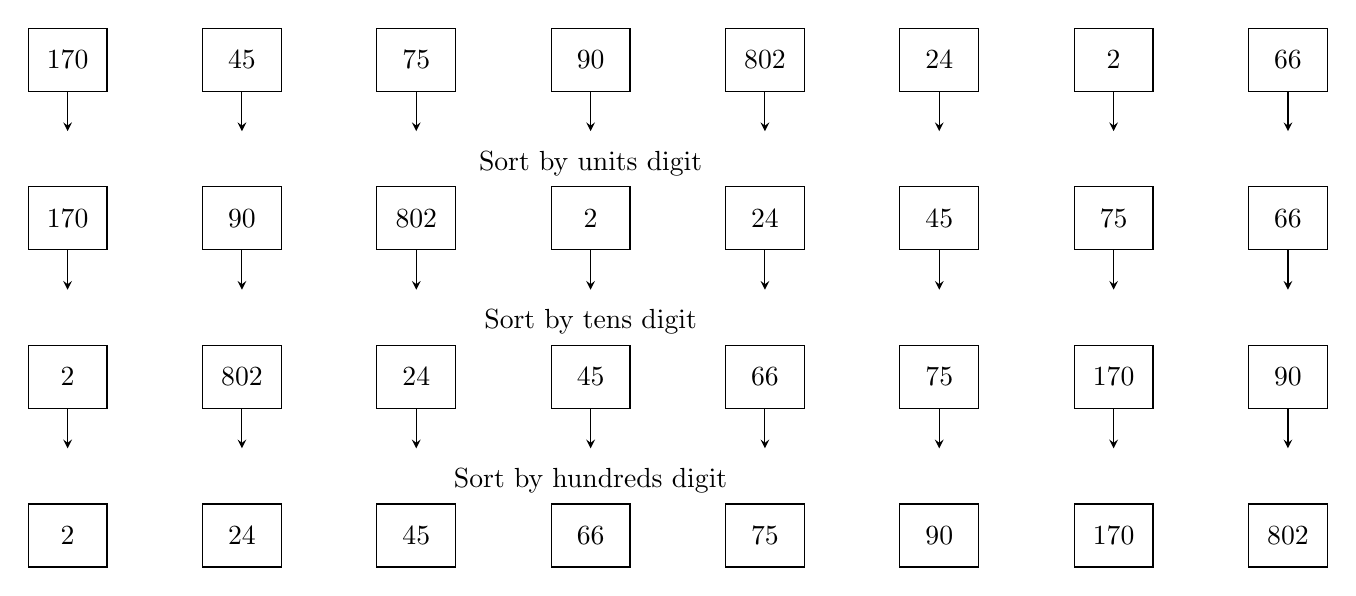
\begin{tikzpicture}[>=stealth, node distance=1.2cm, every node/.style={draw, rectangle, minimum width=1cm, minimum height=0.8cm}]
    % Original array
    \node (n1) {170};
    \node[right=of n1] (n2) {45};
    \node[right=of n2] (n3) {75};
    \node[right=of n3] (n4) {90};
    \node[right=of n4] (n5) {802};
    \node[right=of n5] (n6) {24};
    \node[right=of n6] (n7) {2};
    \node[right=of n7] (n8) {66};

    % Arrow down to units sort
    \node[below=0.5cm of n4, draw=none] (lbl1) {Sort by units digit};
    \draw[->] (n1.south) -- +(0,-0.5);
    \draw[->] (n2.south) -- +(0,-0.5);
    \draw[->] (n3.south) -- +(0,-0.5);
    \draw[->] (n4.south) -- +(0,-0.5);
    \draw[->] (n5.south) -- +(0,-0.5);
    \draw[->] (n6.south) -- +(0,-0.5);
    \draw[->] (n7.south) -- +(0,-0.5);
    \draw[->] (n8.south) -- +(0,-0.5);

    % Sorted by units
    \node[below=1.2cm of n1] (u1) {170};
    \node[right=of u1] (u2) {90};
    \node[right=of u2] (u3) {802};
    \node[right=of u3] (u4) {2};
    \node[right=of u4] (u5) {24};
    \node[right=of u5] (u6) {45};
    \node[right=of u6] (u7) {75};
    \node[right=of u7] (u8) {66};

    % Arrow down to tens sort
    \node[below=0.5cm of u4, draw=none] (lbl2) {Sort by tens digit};
    \draw[->] (u1.south) -- +(0,-0.5);
    \draw[->] (u2.south) -- +(0,-0.5);
    \draw[->] (u3.south) -- +(0,-0.5);
    \draw[->] (u4.south) -- +(0,-0.5);
    \draw[->] (u5.south) -- +(0,-0.5);
    \draw[->] (u6.south) -- +(0,-0.5);
    \draw[->] (u7.south) -- +(0,-0.5);
    \draw[->] (u8.south) -- +(0,-0.5);

    % Sorted by tens
    \node[below=1.2cm of u1] (t1) {2};
    \node[right=of t1] (t2) {802};
    \node[right=of t2] (t3) {24};
    \node[right=of t3] (t4) {45};
    \node[right=of t4] (t5) {66};
    \node[right=of t5] (t6) {75};
    \node[right=of t6] (t7) {170};
    \node[right=of t7] (t8) {90};

    % Arrow down to hundreds sort
    \node[below=0.5cm of t4, draw=none] (lbl3) {Sort by hundreds digit};
    \draw[->] (t1.south) -- +(0,-0.5);
    \draw[->] (t2.south) -- +(0,-0.5);
    \draw[->] (t3.south) -- +(0,-0.5);
    \draw[->] (t4.south) -- +(0,-0.5);
    \draw[->] (t5.south) -- +(0,-0.5);
    \draw[->] (t6.south) -- +(0,-0.5);
    \draw[->] (t7.south) -- +(0,-0.5);
    \draw[->] (t8.south) -- +(0,-0.5);

    % Sorted by hundreds
    \node[below=1.2cm of t1] (h1) {2};
    \node[right=of h1] (h2) {24};
    \node[right=of h2] (h3) {45};
    \node[right=of h3] (h4) {66};
    \node[right=of h4] (h5) {75};
    \node[right=of h5] (h6) {90};
    \node[right=of h6] (h7) {170};
    \node[right=of h7] (h8) {802};
\end{tikzpicture}

\subsection{C++ implementation}

\begin{lstlisting}[style=cppstyle]
// Counting sort by digit represented by exp
void countingSort(int arr[], int n, int exp) {
    int output[n];          // Output array
    int count[10] = {0};    // Count array for digits 0-9

    // Store count of occurrences of each digit
    for (int i = 0; i < n; ++i)
        count[(arr[i] / exp) % 10]++;

    // Update count[i] so it contains actual position of the digit in output
    for (int i = 1; i < 10; ++i)
        count[i] += count[i - 1];

    // Build the output array by placing elements at correct positions
    for (int i = n - 1; i >= 0; --i) {
        int digit = (arr[i] / exp) % 10;
        output[count[digit] - 1] = arr[i];
        count[digit]--;
    }

    // Copy output array back to arr[]
    for (int i = 0; i < n; ++i)
        arr[i] = output[i];
}

// Radix Sort: sorts arr[] using counting sort on each digit
void radixSort(int arr[], int n) {
    int max_val = *std::max_element(arr, arr + n); // Find the maximum number

    // Apply counting sort for each digit place
    for (int exp = 1; max_val / exp > 0; exp *= 10)
        countingSort(arr, n, exp);
}
\end{lstlisting}



 Time Complexity: $O(d \cdot n)$ — linear with respect to input size if $d$ is constant. \\
 Space Complexity: $O(n)$ 





\end{document}